% Options for packages loaded elsewhere
\PassOptionsToPackage{unicode}{hyperref}
\PassOptionsToPackage{hyphens}{url}
%
\documentclass[
  letterpaper,
]{book}

\usepackage{amsmath,amssymb}
\usepackage{lmodern}
\usepackage{iftex}
\ifPDFTeX
  \usepackage[T1]{fontenc}
  \usepackage[utf8]{inputenc}
  \usepackage{textcomp} % provide euro and other symbols
\else % if luatex or xetex
  \usepackage{unicode-math}
  \defaultfontfeatures{Scale=MatchLowercase}
  \defaultfontfeatures[\rmfamily]{Ligatures=TeX,Scale=1}
\fi
% Use upquote if available, for straight quotes in verbatim environments
\IfFileExists{upquote.sty}{\usepackage{upquote}}{}
\IfFileExists{microtype.sty}{% use microtype if available
  \usepackage[]{microtype}
  \UseMicrotypeSet[protrusion]{basicmath} % disable protrusion for tt fonts
}{}
\makeatletter
\@ifundefined{KOMAClassName}{% if non-KOMA class
  \IfFileExists{parskip.sty}{%
    \usepackage{parskip}
  }{% else
    \setlength{\parindent}{0pt}
    \setlength{\parskip}{6pt plus 2pt minus 1pt}}
}{% if KOMA class
  \KOMAoptions{parskip=half}}
\makeatother
\usepackage{xcolor}
\setlength{\emergencystretch}{3em} % prevent overfull lines
\setcounter{secnumdepth}{5}
% Make \paragraph and \subparagraph free-standing
\ifx\paragraph\undefined\else
  \let\oldparagraph\paragraph
  \renewcommand{\paragraph}[1]{\oldparagraph{#1}\mbox{}}
\fi
\ifx\subparagraph\undefined\else
  \let\oldsubparagraph\subparagraph
  \renewcommand{\subparagraph}[1]{\oldsubparagraph{#1}\mbox{}}
\fi


\providecommand{\tightlist}{%
  \setlength{\itemsep}{0pt}\setlength{\parskip}{0pt}}\usepackage{longtable,booktabs,array}
\usepackage{calc} % for calculating minipage widths
% Correct order of tables after \paragraph or \subparagraph
\usepackage{etoolbox}
\makeatletter
\patchcmd\longtable{\par}{\if@noskipsec\mbox{}\fi\par}{}{}
\makeatother
% Allow footnotes in longtable head/foot
\IfFileExists{footnotehyper.sty}{\usepackage{footnotehyper}}{\usepackage{footnote}}
\makesavenoteenv{longtable}
\usepackage{graphicx}
\makeatletter
\def\maxwidth{\ifdim\Gin@nat@width>\linewidth\linewidth\else\Gin@nat@width\fi}
\def\maxheight{\ifdim\Gin@nat@height>\textheight\textheight\else\Gin@nat@height\fi}
\makeatother
% Scale images if necessary, so that they will not overflow the page
% margins by default, and it is still possible to overwrite the defaults
% using explicit options in \includegraphics[width, height, ...]{}
\setkeys{Gin}{width=\maxwidth,height=\maxheight,keepaspectratio}
% Set default figure placement to htbp
\makeatletter
\def\fps@figure{htbp}
\makeatother
\newlength{\cslhangindent}
\setlength{\cslhangindent}{1.5em}
\newlength{\csllabelwidth}
\setlength{\csllabelwidth}{3em}
\newlength{\cslentryspacingunit} % times entry-spacing
\setlength{\cslentryspacingunit}{\parskip}
\newenvironment{CSLReferences}[2] % #1 hanging-ident, #2 entry spacing
 {% don't indent paragraphs
  \setlength{\parindent}{0pt}
  % turn on hanging indent if param 1 is 1
  \ifodd #1
  \let\oldpar\par
  \def\par{\hangindent=\cslhangindent\oldpar}
  \fi
  % set entry spacing
  \setlength{\parskip}{#2\cslentryspacingunit}
 }%
 {}
\usepackage{calc}
\newcommand{\CSLBlock}[1]{#1\hfill\break}
\newcommand{\CSLLeftMargin}[1]{\parbox[t]{\csllabelwidth}{#1}}
\newcommand{\CSLRightInline}[1]{\parbox[t]{\linewidth - \csllabelwidth}{#1}\break}
\newcommand{\CSLIndent}[1]{\hspace{\cslhangindent}#1}

\makeatletter
\makeatother
\makeatletter
\@ifpackageloaded{bookmark}{}{\usepackage{bookmark}}
\makeatother
\makeatletter
\@ifpackageloaded{caption}{}{\usepackage{caption}}
\AtBeginDocument{%
\ifdefined\contentsname
  \renewcommand*\contentsname{Table of contents}
\else
  \newcommand\contentsname{Table of contents}
\fi
\ifdefined\listfigurename
  \renewcommand*\listfigurename{List of Figures}
\else
  \newcommand\listfigurename{List of Figures}
\fi
\ifdefined\listtablename
  \renewcommand*\listtablename{List of Tables}
\else
  \newcommand\listtablename{List of Tables}
\fi
\ifdefined\figurename
  \renewcommand*\figurename{Figure}
\else
  \newcommand\figurename{Figure}
\fi
\ifdefined\tablename
  \renewcommand*\tablename{Table}
\else
  \newcommand\tablename{Table}
\fi
}
\@ifpackageloaded{float}{}{\usepackage{float}}
\floatstyle{ruled}
\@ifundefined{c@chapter}{\newfloat{codelisting}{h}{lop}}{\newfloat{codelisting}{h}{lop}[chapter]}
\floatname{codelisting}{Listing}
\newcommand*\listoflistings{\listof{codelisting}{List of Listings}}
\makeatother
\makeatletter
\@ifpackageloaded{caption}{}{\usepackage{caption}}
\@ifpackageloaded{subcaption}{}{\usepackage{subcaption}}
\makeatother
\makeatletter
\@ifpackageloaded{tcolorbox}{}{\usepackage[many]{tcolorbox}}
\makeatother
\makeatletter
\@ifundefined{shadecolor}{\definecolor{shadecolor}{rgb}{.97, .97, .97}}
\makeatother
\makeatletter
\makeatother
\ifLuaTeX
  \usepackage{selnolig}  % disable illegal ligatures
\fi
\IfFileExists{bookmark.sty}{\usepackage{bookmark}}{\usepackage{hyperref}}
\IfFileExists{xurl.sty}{\usepackage{xurl}}{} % add URL line breaks if available
\urlstyle{same} % disable monospaced font for URLs
\hypersetup{
  pdftitle={Introduction to Digital History},
  pdfauthor={Ina Serif},
  hidelinks,
  pdfcreator={LaTeX via pandoc}}

\title{Introduction to Digital History}
\author{Ina Serif}
\date{}

\begin{document}
\frontmatter
\maketitle
\ifdefined\Shaded\renewenvironment{Shaded}{\begin{tcolorbox}[interior hidden, boxrule=0pt, borderline west={3pt}{0pt}{shadecolor}, frame hidden, breakable, sharp corners, enhanced]}{\end{tcolorbox}}\fi

\renewcommand*\contentsname{Table of contents}
{
\setcounter{tocdepth}{2}
\tableofcontents
}
\mainmatter
\bookmarksetup{startatroot}

\hypertarget{welcome}{%
\chapter*{Welcome}\label{welcome}}
\addcontentsline{toc}{chapter}{Welcome}

\markboth{Welcome}{Welcome}

Der vorliegende Guide begleitet die Einführungskurse im Fach Geschichte
an der Universität Basel und soll einen ersten Einblick in den Bereich
digital history geben. Die epochen- und areaspezifischen Inhalte der
verschiedenen Einführungskurse sollen dabei berücksichtigt werden, die
Verweise auf verschiedene digital-history-Projekte aus unterschiedlichen
Epochen mit der Zeit also anwachsen.

Der Guide wird für die Teilnehmer:innen der Einführungskurse von einer
Präsenzsitzung begleitet, bietet aber hoffentlich auch unabhängig davon
einen Mehrwert. Für Kommentare, Anregungen oder Beschwerden freue ich
mich über eine Nachricht.

Der Guide ist in zwei Teile gegliedert: Die Kapitel 1--5 sollen eine
erste Übersicht über ``digital history'' bieten und den Blick auf
Neuerungen und Veränderungen richten, die sich in den
Geschichtswissenschaften aus der Nutzung digitaler Methoden ergeben. Der
anschließende Praxisteil zeigt an einem konkreten Beispiel die Anwendung
verschiedener Techniken auf, die sich (nicht nur) für Historiker:innen
bei der Arbeit mit Quellenmaterial anbieten. Der Praxisteil verfolgt
dabei zwei Ziele: Zum einen sollen Hemmungen bei der Arbeit mit dem
Computer, die über die Nutzung als elektronische Schreibmaschine
hinausgeht, abgebaut werden. Zum zweiten sollen ein grundlegendes
Verständnis dafür hergestellt werden, welche Möglichkeiten
computergestützte Analysen bieten und wie diese in der historischen
Arbeit eingesetzt werden können.

Die Übersicht soll möglichst knapp gehalten werden -- es gibt zahlreiche
ausführliche Grundlagenwerke, weswegen viele Themen nur kurz
angeschnitten, dafür aber mit weiterführenden Verweisen versehen werden.
Dasselbe gilt für den Praxisteil: Weiterreichende Anleitungen, Tutorials
oder Onlinekurse werden an entsprechender Stelle verlinkt.
Vollständigkeit wird an keiner Stelle beansprucht; Hinweise auf weitere
Online-Angebote nehme ich gerne auf.

\bookmarksetup{startatroot}

\hypertarget{was-ist-digital-history}{%
\chapter{Was ist digital history?}\label{was-ist-digital-history}}

Über die Antwort zur Frage, was digital history ist oder umfasst, kann
man ausgiebig diskutieren; als Teilgebiet der digital humanities, der
digitalen Geisteswissenschaften, kann die folgende aktuelle und
pragmatische Definition von Blaney et al.~hilfreich sein:

\begin{quote}
Digital humanities, in our view, is a question of approach: if you are
actively and critically using digital tools to aid your work in
researching, teaching or learning, you are probably doing digital
humanities. We would encourage anyone to learn to program if they are
interested in doing so, but we do not see it as a defining
characteristic of work in digital humanities.\footnote{Blaney, Jonathan;
  Winters, Jane; Milligan, Sarah u.~a.: Doing digital history: a
  beginner's guide to working with text as data, Manchester 2021 ({IHR}
  research guides), S.~6.}
\end{quote}

Dabei umfassen ``digital tools'' eine große Bandbreite -- und es wird
sich kaum eine:r finden, der:die Studium, Forschung oder Lehre völlig
ohne die Nutzung digitaler Techniken betreibt. Wir sind alle
Historiker:innen im digitalen Zeitalter, und als solche müssen wir
ohnehin neue Kompetenzen entwickeln. Wir können uns aber zudem dafür
entscheiden, für ein Forschungsprojekt Methoden und Techniken
einzusetzen, die über die traditionellen Werkzeuge der
Geschichtswissenschaften hinausgehen -- Analyse und Interpretation von
Quellen durch deren genaue Lektüre, sogenanntes \emph{close reading} --,
und uns durch den Computer unterstützen lassen. Ob wir hierbei auf
vorhandene Software zurückgreifen oder selbst Programme schreiben, um
uns nicht nur als Historiker:innen im digitalen Zeitalter, sondern auch
als digitale Historiker:innen zu verstehen, mögen manche als
Glaubensfrage auffassen; eine inkludierende Haltung zu dieser Frage
scheint mir dabei nur Vorteile zu haben.\footnote{Entgegen einer häufig
  zitierten Aussage von Emmanuel Le Roy Ladurie (*1929), der Historiker
  von morgen werde Programmierer sein, oder er werde nicht sein:
  ``L'historien de demain sera programmeur ou il ne sera pas.'' Le Roy
  Ladurie, Emmanuel: La fin des {é}rudits, in: Le Nouvel Observateur,
  08.1968.}

Für eine erste Idee dafür, wie man historische Fragestellungen mithilfe
digitaler Methoden beantworten kann und wie unterschiedlich digital
unterstützte Forschungsprojekte aussehen können, bietet sich unter
anderem der Übersichtsartikel
``\href{https://onlinelibrary.wiley.com/doi/10.1111/1468-229X.12969}{State
of the Field: Digital History}'' von Romein et al.~(2020) an.\footnote{Romein,
  C. Annemieke; Kemman, Max; Birkholz, Julie M. u.~a.: State of the
  {Field}: {Digital} {History}, in: History 105~(365), 04.2020,
  S.~291--312. Online:
  \textless{}\url{https://doi.org/10.1111/1468-229X.12969}\textgreater,
  Stand: 15.09.2022.} Eine anwachsende Liste an Beispielprojekten aus
unterschiedlichen Epochen bzw. Themenbereichen findet sich in
Section~\ref{sec-projects}.

Um eine Annäherung an die aktive, kritische und reflektierte Nutzung
digitaler Methoden in Forschung und Lehre mit einem Fokus auf deren
Anwendung in den Geschichtswissenschaften geht es im vorliegenden Guide.
Weiterführende Texte zur Frage, was digital history ist bzw. umfasst,
finden sich in \textbf{?@sec-digitalhistory-paper}.

\bookmarksetup{startatroot}

\hypertarget{forschung-und-lehre}{%
\chapter{Forschung und Lehre}\label{forschung-und-lehre}}

Die fortschreitende Digitalisierung in ganz unterschiedlichen
Lebensbereichen zieht Veränderungen und Entwicklungen auch für die
historische Arbeit mit sich, und dies auf mehreren Ebenen: in Bezug auf
die Arbeit bzw. den Umgang mit Quellen, hinsichtlich des Einsatzes
digitaler Methoden nicht nur zur Kommunikation von
Forschungsergebnissen, sondern auch für deren Analyse, und schließlich
für die Hochschullehre.

\begin{figure}

\href{history_department}{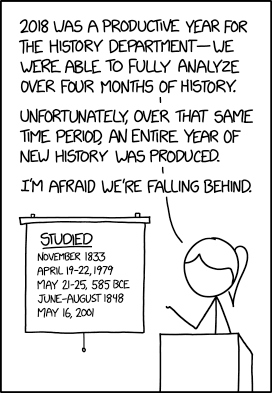
\includegraphics{https://imgs.xkcd.com/comics/history_department.png}}

\caption{Randall Munroe, History Department, xkcd.com (17.12.2018).}

\end{figure}

Als Historiker:innen steht die Arbeit mit Quellen im Mittelpunkt unserer
Analysen. Das bedeutet gleichzeitig, dass der Zugang bzw. die
Verfügbarkeit von Dokumenten einen Einfluss darauf hat, welche Fragen
wir beantworten oder welche Analysen wir vornehmen können.
Zugangsbeschränkungen, die die Größe und Zusammensetzung unseres
Untersuchungskorpus beeinflussen, können dabei von
Gedächtnisinstitutionen ausgehen, beispielsweise wenn bei
zeitgenössischen Akten eine Schutzfrist festgesetzt wird oder wenn ein
Objekt zu fragil für die Benutzung ist. Auch kann es aus finanziellen
und/oder organisatorischen Gründen schwierig sein, bestimmte Archive an
weiter entfernten Orten aufzusuchen, um weitere Dokumente für die
Untersuchung zu berücksichtigen. Groß angelegte Digitalisierungsprojekte
in Bibliotheken und Archiven bergen damit die Möglichkeit, zusätzliche
Quellen nicht nur über einen Eintrag im Bibliothekskatalog zu finden,
sondern die entsprechenden Dokumente in digitaler Form auf den eigenen
Rechner zu laden. Gerade auch für wertvolle historische Bestände --
antike Papyri, Handschriften aus dem Frühmittelalter, einzelüberlieferte
Frühdrucke usw. -- entsteht hier die Möglichkeit, diese einem größeren
Kreis verfügbar zu machen, ohne das Objekt zu großer Belastung durch
häufige Benutzung auszusetzen, und ohne dass die Benutzer:innen lange
Reisen auf sich nehmen müssten. Für mittelalterliche und
frühneuzeitliche Handschriften und Drucke beispielsweise existieren
mittlerweile mehrere (meist nationale) Portale, die eine zentrale Suche
über alle Bestände ermöglichen; eine Auswahl findet sich in
Section~\ref{sec-projects-ma-fnz}.

Neben der Digitalisierung vorhandener Quellen (Retrodigitalisierung)
steht die unaufhörliche Entstehung neuer Quellen in rein digitaler Form
(born digital data). Die relative Knappheit von Quellen -- und damit
Daten --, die die Vormodernehistorikerin oftmals zu beklagen hat, steht
einer Überfülle an zeitgenössischem Material gegenüber, und beide
Situationen -- zu wenig/zu unvollständige und zu viele/zu
unübersichtliche Datenmengen -- bergen methodische Probleme: Wie stellt
man ein Korpus zusammen, das ausreichend Quellen beinhaltet, um
Fragestellungen zu beantworten, Thesen zu stützen, neue Erkenntnisse zu
erhalten, das aber gleichzeitig in einem Forscherinnenleben bewältigbar
bleibt?

Bei beiden Quellenarten, den retrodigitalisierten wie den rein
digitalen, stellt sich also die Frage der Korpusbildung, die mit einer
Quellenkritik einhergeht: Woher kommt eine Quelle, wer hat sie unter
welchen Umständen und zu welchem Zweck erstellt? Welche Tendenzen können
darin verborgen sein, und welche Verzerrungen können sich durch sie
ergeben? Bei analogen Quellen, die auch in digitaler Form zur Verfügung
stehen, besteht die Gefahr, dass ein Thema, ein Bereich, ein Aspekt
vernachlässigt wird, wenn nur die unmittelbar verfügbaren,
digitalisierten Bestände zur Korpusbidlung genutzt werden. Wenn Sie sich
beispielsweise für die Schweizer Historikerin und Frauenrechtlerin
\href{https://de.wikipedia.org/wiki/Meta_von_Salis}{Meta von Salis}
(1855--1929) und deren briefliche Korrespondenz -- Friedrich Nietzsche
war einer ihrer Brieffreunde -- interessieren und über die Suchplattform
für historische Schweizer Bestände,
\href{https://swisscollections.ch/Search/Advanced}{swisscollections}, in
nationalen Bibliotheken und Archiven nach entsprechenden Dokumenten
suchen, erhalten Sie 361 Treffer:

\begin{figure}

\begin{minipage}[t]{0.49\linewidth}

{\centering 

\raisebox{-\height}{

\href{_book}{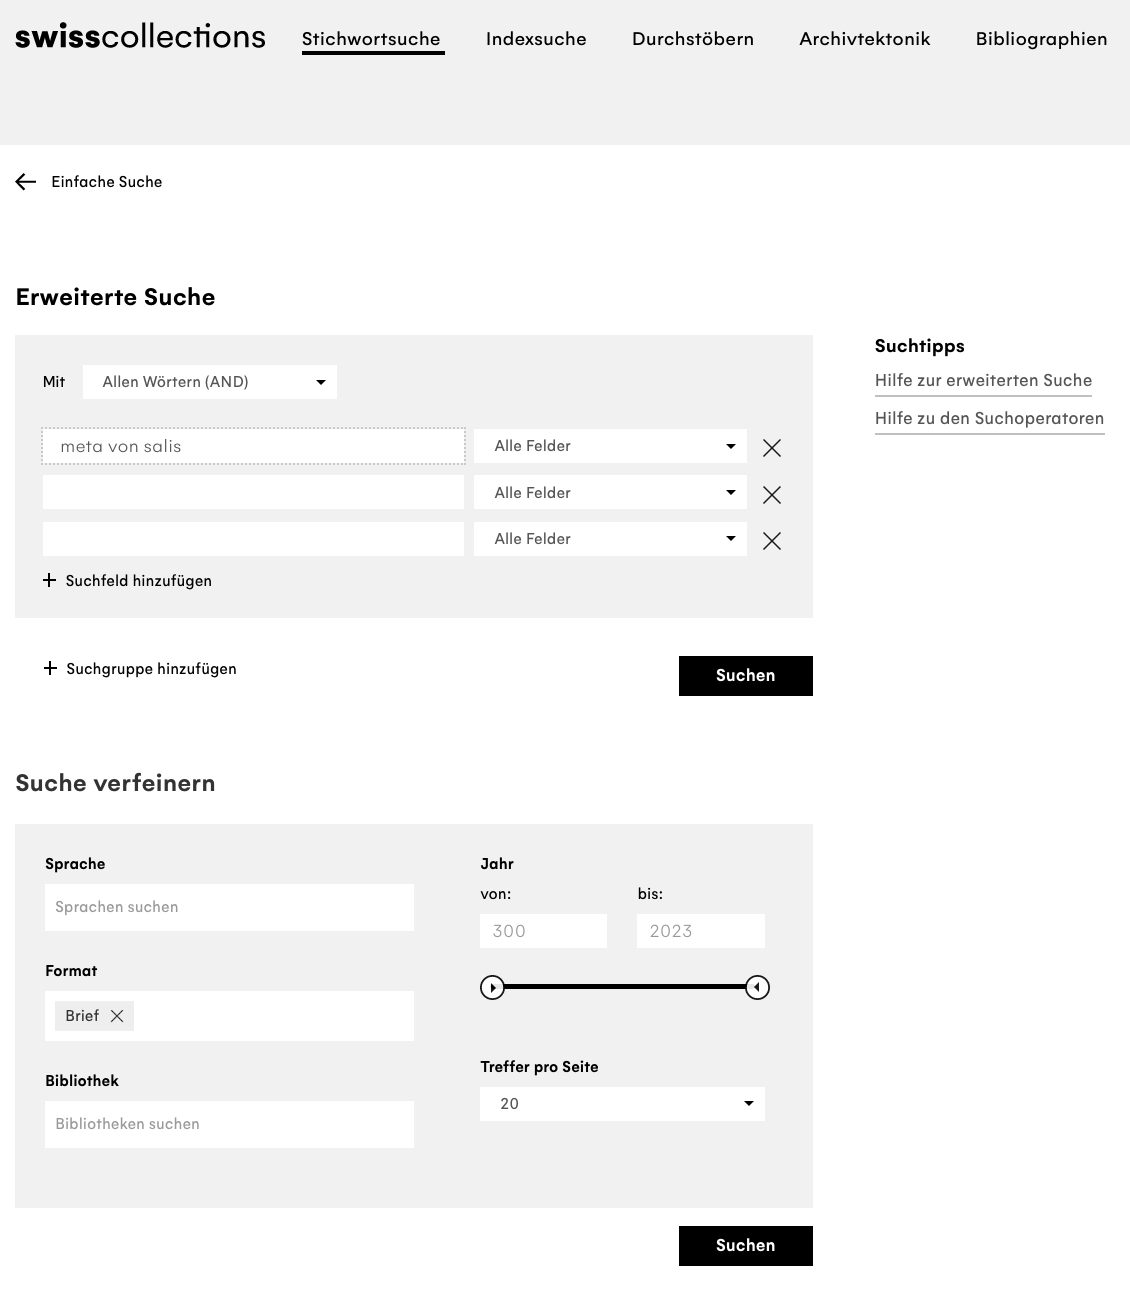
\includegraphics{./_book/images/suche_meta_von_salis.png}}

}

\caption{Erweiterte Suchmaske von swisscollections}

}

\end{minipage}%
%
\begin{minipage}[t]{0.02\linewidth}

{\centering 

~

}

\end{minipage}%
%
\begin{minipage}[t]{0.49\linewidth}

{\centering 

\raisebox{-\height}{

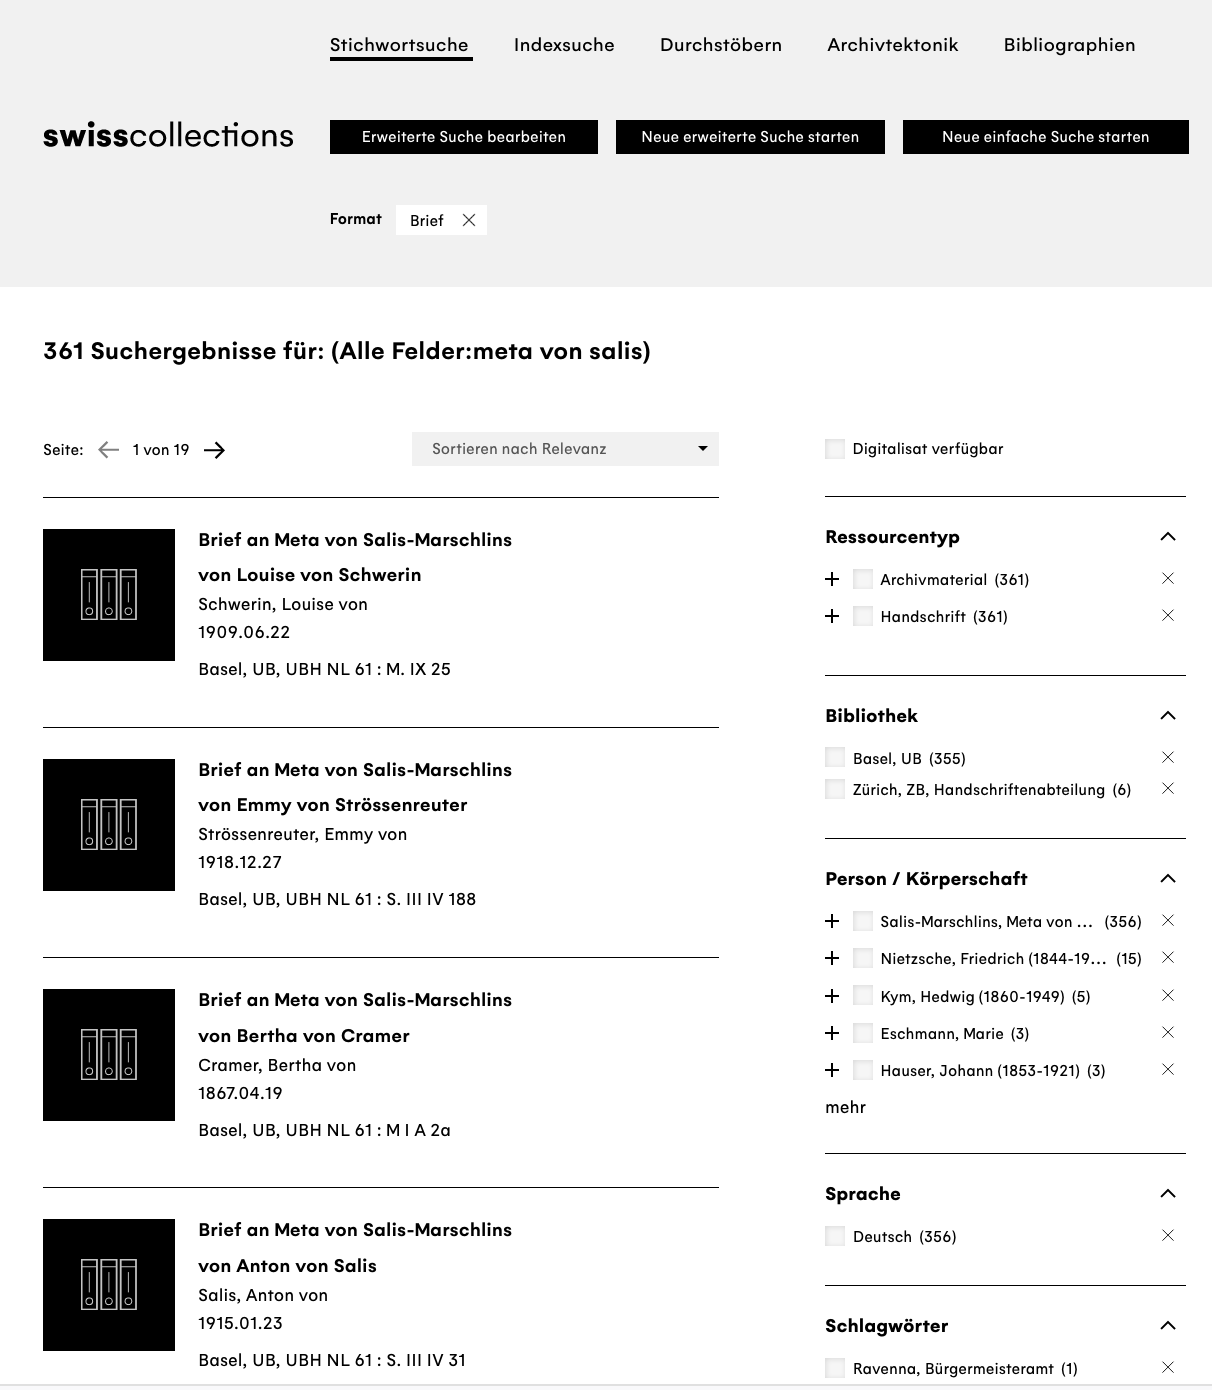
\includegraphics{./_book/images/suchergebnisse_1.png}

}

\caption{Suchergebnisse für ``Meta von Salis'' + ``Brief''}

}

\end{minipage}%

\end{figure}

Digital verfügbar waren hiervon im Oktober 2022 lediglich 3 Einträge,
wobei der erste ein Brief von Nietzsche an Meta von Salis ist, der
zweite Eintrag umfasst sieben Briefe von Caroline Farner, der dritte
Eintrag ist weder an noch von Meta von Salis, sondern hat sie nur zum
Thema:

\begin{figure}

{\centering 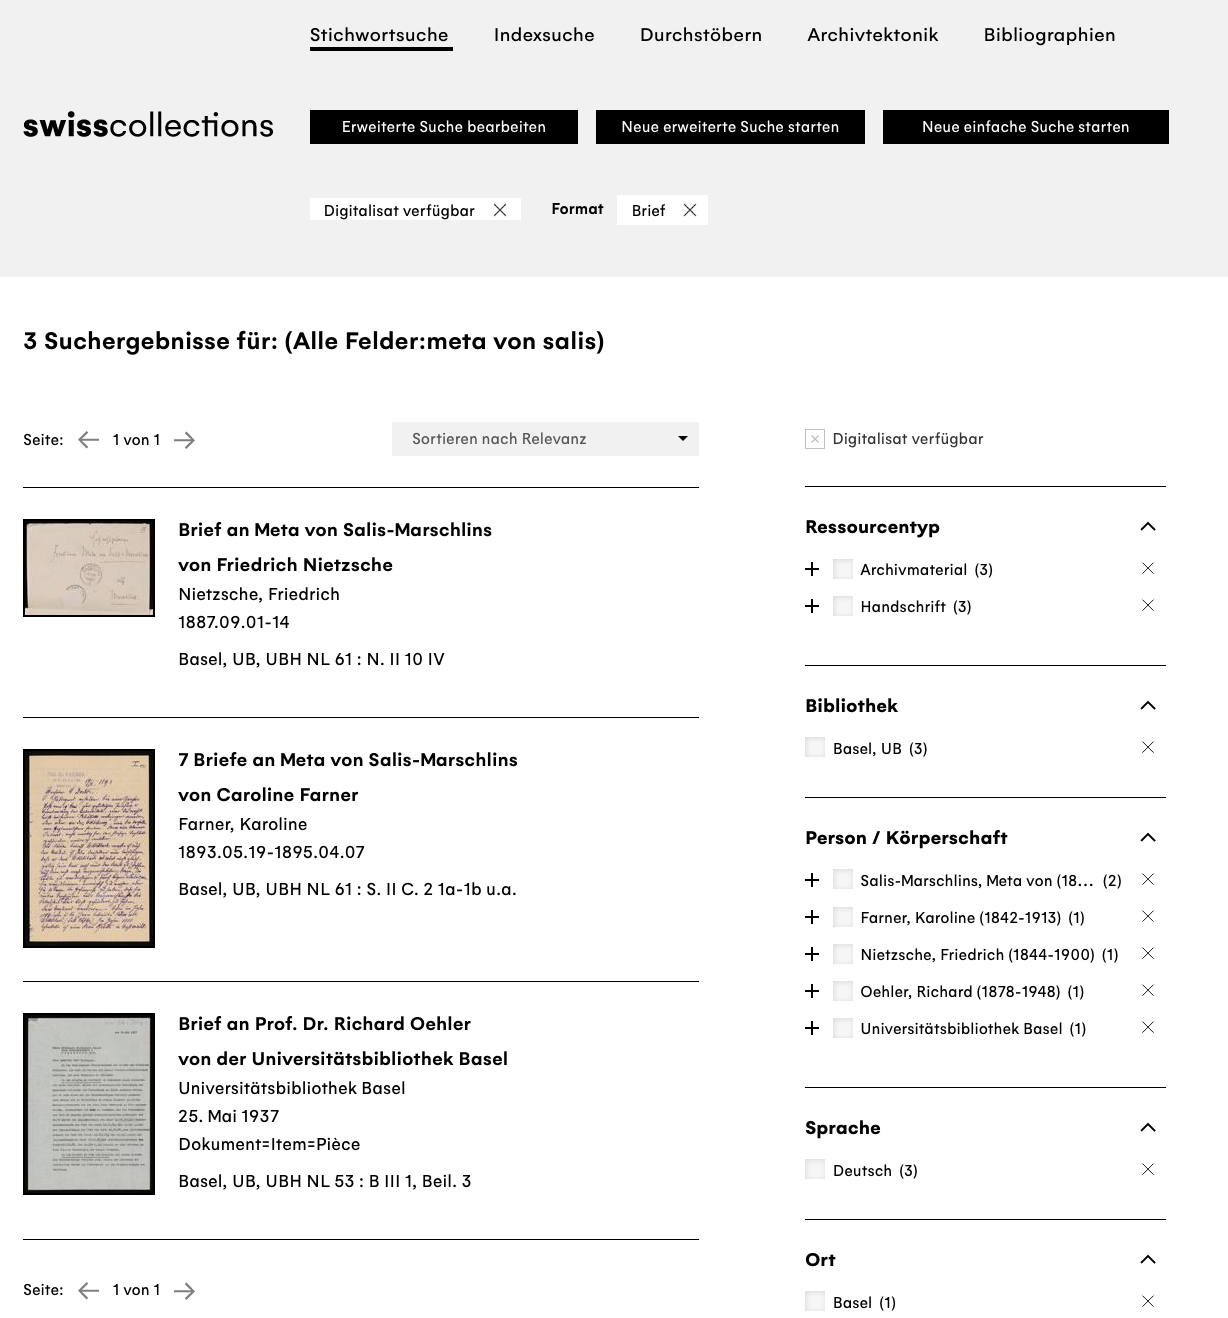
\includegraphics{./_book/images/suchergebnisse_2.png}

}

\caption{Suchergebnisse für ``Meta von Salis'' + ``Brief'' +
``Digitalisat verfügbar''}

\end{figure}

Ihnen würde bei einer Korpuserstellung vom Schreibtisch aus also der
Großteil der Überlieferung fehlen, und Ihre Untersuchungsergebnisse
wären wohl sehr verzerrt, würden Sie statistische Aussagen treffen
wollen: Meta von Salis unterhielt brieflichen Kontakt zu einem Mann und
einer Frau, das Geschlechterverhältnis wäre also ausgeglichen; und
Frauen schreiben im Schnitt mehr Briefe an Meta von Salis als Männer.
Beim Blick auf alle Suchergebnisse würden sich Ihre Aussagen aber sehr
ändern, und es würde sich lohnen, diese Verzerrung, diesen Bias aus
Ihrer Datengrundlage zu entfernen.

\begin{quote}
Hinzu kommt natürlich immer das grundlegende Problem bei der Suche nach
Quellen: swisscollections und ähnliche Portale können nur anzeigen, was
die Kooperationspartner:innen zur Verfügung stellen. Hat eine Bibliothek
Briefe von Meta von Salis in ihrem Bestand, diese aber noch nicht als
Datensatz erfasst, wissen Sie im Gegensatz zum obigen Beispiel nicht
einmal, dass Ihnen etwas entgehen würde, dass in Ihrem Korpus überhaupt
ein Bias vorhanden ist.
\end{quote}

Ähnliche Vorsicht zur Vermeidung von Verzerrungen in der Datengrundlage
gilt bei der Arbeit mit rein digitalen Daten, beispielweise bei der
Auswertung von Datensätzen aus Befragungen. Wenn Sie sich am 27.10.2022
vor die Universitätsbibliothek in Basel stellen und einen Tag lang
mithilfe eines kurzen Fragebogens und einer Tabellendatei erfassen, wie
zufrieden die befragten Personen mit dem Essen in der Unimensa sind,
werden Sie am Ende einen Datensatz erhalten, in dem sich vermutlich über
80\% der Befragten für besseres und nahezu 100\% für günstigeres Essen
in der Mensa aussprechen -- eine gute Schlagzeile für die BZ, die sich
auf die neuesten Ergebnisse einer wissenschaftlichen Studie berufen
kann. Führen Sie die gleiche Umfrage eine Woche später, mitten während
der Herbstmesse durch, werden die Ergebnisse wohl erheblich anders
aussehen. Die Wahrscheinlichkeit, dass die Mensa infolge der
BZ-Schlagzeile innerhalb weniger Tage den Menüplan überarbeitet und die
Preise herabgesetzt hat, ist dabei wohl geringer als diejenige, dass
sich Ihr Sample, die Auswahl an Datenpunkten, also befragten Personen,
durch die Messe stark verändert hat: Im Umkreis der Bibliothek treffen
Sie nun nicht mehr vor allem Studierende und andere Uni-Angehörige an,
sondern auch Messebesucher:innen vom Petersplatz. Auch hier sind
Verzerrungen entstanden, ähnlich wie beim vorherigen Beispiel mit den
Briefen: Wenn aus einer Gesamtheit nur eine spezifische Untermenge
beobachtet wird, die sich durch ein gemeinsames Merkmal von der
Gesamtheit unterscheidet -- digitalisierte Quelle oder Besucher:in der
Universitätsbibliothek --, ist die Datengrundlage und damit die
Untersuchungsergebnisse biased.

Bias finden Sie überall, und er wird sich nie ganz vermeiden lassen,
aber ein reflektierter Umgang damit ist eine wichtige Voraussetzung für
die Analyse von Daten und die Interpretation von Resultaten: Gehen Sie
auf die \href{https://images.google.com/}{Bilder-Suche von Google} und
suchen Sie nach ``historian''.

Wüsste ich nichts über Geschichtswissenschaftler:innen, würde ich
aufgrund der Ergebnisse meiner Suche davon ausgehen, ``a historian''
wäre meist ein alter, weißer Mann mit Brille, Bart und einem großen
Bücherregal; wenn Sie sich am Departement Geschichte der Uni Basel
umsehen, dürfte ein etwas anderer Eindruck entstehen. Aber auch die
Ergebnisse von Suchmaschinen, die für ihr Funktionieren Algorithmen
anwenden, sind biased: Sie beruhen auf vorangegangenen Suchen,
Vorlieben, geographischem Standort -- und auf von Menschen eingegebenen
Metadaten. Ein Bewusstsein hierfür und das Hinterfragen von Datensätzen
gehören also mit zur Arbeit in einer digitalisierten Welt.

Zur Tatsache, dass Daten eben nicht gegeben sind (lat. dare, datum:
gebene, gegeben), sondern gemacht und daher entsprechend interpretiert
werden müssen, finden Sie ein gutes Interview von Roopika
Risam;\footnote{Risam, Roopika: {``}{It}{'}s {Data}, {Not}
  {Reality}{''}: {On} {Situated} {Data} {With} {Jill} {Walker}
  {Rettberg}, 06.2020. Online:
  \textless{}\url{https://medium.com/nightingale/its-data-not-reality-on-situated-data-with-jill-walker-rettberg-d27c71b0b451}\textgreater,
  Stand: 16.08.2022.}; zur Zementierung von Klischees durch
Übersetzungsalgorithmen gibt es einen Artikel in der Republik von
Marie-José Kolly und Simon Schmid;\footnote{Kolly, Marie-José; Schmid,
  Simon: Sie ist h{ü}bsch. {Er} ist stark. {Er} ist {Lehrer}. {Sie} ist
  {Kinderg{ä}rtnerin}, in: Republik, 04.2021. Online:
  \textless{}\url{https://www.republik.ch/2021/04/19/sie-ist-huebsch-er-ist-stark-er-ist-lehrer-sie-ist-kindergaertnerin}\textgreater,
  Stand: 23.08.2022.} und über die Macht von Data Science und dem
Änderungspotential von Data Feminism haben Cathherine D'Ignazio und
Lauren F. Klein ein ganzes Buch veröffentlich.{[}dignazio\_data\_2020{]}

Zur Frage, wie sich die digitale Wende, der digital turn, auf die
Quellenkritik auswirkt, sehen Sie sich dieses kurze Video des Projekts
\href{https://ranke2.uni.lu}{Ranke.2 -- Quellenkritik im digitalen
Zeitalter} an\footnote{Kommandozeile/command line, bash, shell, prompt
  finden sich oft als synonym genutzte Begriffe für Command Line
  Interfaces. Auf UNIX-basierten Betriebssystemen wie Mac OS und Linux
  ist das Terminal als Interface weit verbreitet; für Details:
  https://en.wikipedia.org/wiki/Command-line\_interface\#History.
  Windowsnutzer:innen kommen mit der Powershell ganz gut zurecht, es
  empfiehlt sich eventuell die Installation von
  \href{https://en.wikipedia.org/wiki/Cygwin}{Cygwin} oder
  \href{https://en.wikipedia.org/wiki/MinGW}{MinGW}, um mit einem
  UNIX-basierten Interface arbeiten zu können.}:

Eine Handreichung zum Umgang mit digitalisierten und digitalen Daten,
das im selben Projekt erarbeitet wurde, finden Sie
\href{_book/documents/Ranke_visual-aid.pdf}{hier}.

\hypertarget{digitale-tools-zur-kommunikation}{%
\section{Digitale Tools zur
Kommunikation}\label{digitale-tools-zur-kommunikation}}

\hypertarget{digitale-tools-zur-analyse}{%
\section{Digitale Tools zur Analyse}\label{digitale-tools-zur-analyse}}

\hypertarget{digitale-elemente-in-der-hochschullehre}{%
\section{Digitale Elemente in der
Hochschullehre}\label{digitale-elemente-in-der-hochschullehre}}

\hypertarget{sec-projects}{%
\section{Projekte und Ressourcen}\label{sec-projects}}

\hypertarget{alte-geschichte}{%
\subsection{Alte Geschichte}\label{alte-geschichte}}

Projekte:

Ressourcen/Portale:

\hypertarget{sec-projects-ma-fnz}{%
\subsection{Mittelalter und Frühe Neuzeit}\label{sec-projects-ma-fnz}}

Projekte:

Ressourcen/Portale:

\begin{itemize}
\item
  \href{https://www.e-codices.unifr.ch/de}{e-codices: Virtuelle
  Handschriftenbibliothek der Schweiz}
\item
  \href{https://fragmentarium.ms/}{Fragmentarium: Laboratory for
  Medieval Manuscript Fragments}
\item
  \href{https://handschriftenportal.de/}{Handschriftenportal: Zentraler
  nationaler Nachweis für Buchhandschriften in deutschen Bibliotheken
  und in deutscher Sprache (Entwicklungsstadium)}
\item
  \href{https://www.e-manuscripta.ch/?lang=de}{e-manuscripta:
  Digitalisierte handschriftliche Quellen aus Schweizer Bibliotheken und
  Archiven}
\item
  \href{https://www.e-rara.ch/?lang=de}{e-rara: Plattform für
  digitalisierte Drucke aus Schweizer Institutionen}
\end{itemize}

\hypertarget{moderne-und-zeitgeschichte}{%
\subsection{Moderne und
Zeitgeschichte}\label{moderne-und-zeitgeschichte}}

Projekte:

Ressourcen/Portale:

\hypertarget{juxfcdische-geschichte}{%
\subsection{Jüdische Geschichte}\label{juxfcdische-geschichte}}

Projekte:

\begin{itemize}
\tightlist
\item
  \href{https://jewishstudies.washington.edu/digital-jewish-studies/}{Digital
  Jewish Studies Online}, Stroum Center for Jewish Studies, University
  of Washington
\end{itemize}

Ressourcen/Portale:

\begin{itemize}
\tightlist
\item
  Menny, Anna; Rürup, Miriam; Siegel, Björn: Jüdische Geschichte im
  deutschsprachigen Raum, in: Busse, Laura u.~a.~(Hg.): Clio-Guide. Ein
  Handbuch zu digitalen Ressourcen für die Geschichtswissenschaften,
  Berlin 2018, S. E.2-1--E.2-56. Online:
  \url{https://doi.org/10.18452/19244}.
\end{itemize}

\hypertarget{geschichte-afrikas}{%
\subsection{Geschichte Afrikas}\label{geschichte-afrikas}}

Projekte:

Ressourcen/Portale:

\hypertarget{osteuropuxe4ische-geschichte}{%
\subsection{Osteuropäische
Geschichte}\label{osteuropuxe4ische-geschichte}}

Projekte:

Ressourcen/Portale:

\hypertarget{epochen-areauxfcbergreifend}{%
\subsection{Epochen-/Areaübergreifend:}\label{epochen-areauxfcbergreifend}}

Projekte:

Ressourcen/Portale:

\begin{itemize}
\tightlist
\item
  \href{https://arounddh.org/index.html}{Around DH in 80 days}
\end{itemize}

\bookmarksetup{startatroot}

\hypertarget{shell}{%
\chapter{shell}\label{shell}}

Shell 101

Es gibt zwei Arten, um mit dem Computer zu interagieren bzw. ihn zu
nutzen: über ein \textbf{G}raphical \textbf{U}ser \textbf{I}nterface
(GUI) oder, etwas direkter, über die
\href{https://de.wikipedia.org/wiki/Kommandozeile}{Kommandozeile}\footnote{Kommandozeile/command
  line, bash, shell, prompt finden sich oft als synonym genutzte
  Begriffe für Command Line Interfaces. Auf UNIX-basierten
  Betriebssystemen wie Mac OS und Linux ist das Terminal als Interface
  weit verbreitet; für Details:
  https://en.wikipedia.org/wiki/Command-line\_interface\#History.
  Windowsnutzer:innen kommen mit der Powershell ganz gut zurecht, es
  empfiehlt sich eventuell die Installation von
  \href{https://en.wikipedia.org/wiki/Cygwin}{Cygwin} oder
  \href{https://en.wikipedia.org/wiki/MinGW}{MinGW}, um mit einem
  UNIX-basierten Interface arbeiten zu können.}. Um eine Datei
``Bild1.jpg'' im Ordner ``Bilder'' zu löschen, öffnet man den Explorer
(Windows) oder den Finder (Mac), klickt sich zum Ordner ``Bilder'',
macht einen Rechtsklick auf die zu löschende Datei ``Bild1.jpg'', klickt
``In den Papierkorb legen'' oder zieht die Datei mit der Maus direkt
dorthin. Man kann dieselbe Aktion als Kommando eintippen: Man öffnet
eine Powershell (Windows) oder das Terminal (Mac), navigiert mit
Texteingabe zum entsprechenden Ordner, bspw.
\texttt{cd\ Dokumente/Bilder} und gibt dort das Kommando
\texttt{rm\ "Datei.jpg"} ein, das mit der Entertaste ausgeführt wird.

\texttt{(base)\ serina00@dg-19-mac-02\ Bilder\ \%\ rm\ "Datei.jpg"}

Die beiden Vorgehensweisen unterscheiden sich dabei in drei Punkten:

\begin{enumerate}
\def\labelenumi{\arabic{enumi}.}
\tightlist
\item
  Das Kommando \texttt{rm} ist endgültig, die Datei ist ohne
  Übergangszeit im Papierkorb gelöscht.
\item
  Das Kommando lässt sich relativ simpel auf eine Vielzahl von
  Dokumenten anwenden, wobei ganz unterschiedliche Bedingungen beachtet
  werden können, und es lässt sich mit anderen Kommandos verbinden.
\item
  Terminal sieht k3wl aus.
\end{enumerate}

Bevor wir den zweiten -- und für unsere Arbeit hilfreichsten --
Unterschied genauer anschauen, kurz zur Kommandozeile:

In einem Terminal/Shell können Befehle/Programme ausgeführt werden, die
auf der Datenstrukturebene stattfinden -- wie beispielsweise das Löschen
einer Datei, \texttt{rm\ Dateiname.xyz}, oder das Erstellen eines
Ordners, \texttt{mkdir\ NeuerOrdner}. Oder aber Operationen auf
Dateninhaltsebene -- wie beispielsweise das Suchen eines bestimmten
Begriffs in einer Textdatei, \texttt{grep\ Begriff\ Textdatei.txt}, oder
das Auszählen mehrerer Begriffe und das Speichern des Ergebnisses in
einer neuen Datei,
\texttt{grep\ -Ec\ "Begriff1\textbar{}Begriff2"\ Textdatei.txt\ \textgreater{}\ Ergebnisse.txt}.

Woher weiss Ihre Shell aber, was sie ausführen soll, wenn Sie
\texttt{rm} oder \texttt{grep} eintippen? Es gibt zahlreiche
Shell-Programme, die bereits auf Ihrem System vorinstalliert sind, und
mit denen Sie vieles tun können -- öffnen Sie Ihre Shell und tippen Sie
\texttt{date} ein: Das aktuelle Datum mit Uhrzeit erscheint. Ihre Shell
sucht nach dem ersten Argument, dem Befehl, im Filesystem des Computers,
und wenn sie fündig wird, führt sie eine Aktion mit den entsprechenden
Parametern aus.

\begin{quote}
tmi: Wenn Sie \texttt{echo\ \$PATH} im Terminal eingeben, sehen Sie eine
Auflistung der Orte, an denen nach Befehlen gesucht wird. Tippen Sie
\texttt{which\ date} ein und drücken Sie `Enter', um zu sehen, wo das
Programm ``date'' in Ihrem Computer liegt.
\end{quote}

Wenn Sie einen Befehl eintippen, den es nicht gibt bzw. für den es noch
kein installiertes Programm auf Ihrem Computer gibt, bekommen Sie eine
simple Fehlermeldung:

\texttt{(base)\ serina00@dg-19-mac-02\ EK-dh\ \%\ nonsense}

\texttt{command\ not\ found:\ nonsense}

Das aktuelle Datum wird Ihnen wahrscheinlich auch in Ihrer Toolbar
angezeigt, und einen neuen Ordner können Sie per Rechtsklick erstellen,
dazu brauchen Sie das Terminal nicht unbedingt. Um einen Begriff in
einem Textdokument zu finden und alle Vorkommen zu zählen, können Sie
das Dokument öffnen, \texttt{Strg-F} drücken, den Begriff eingeben und
das Ergebnis sehen. Wenn Sie nach mehreren Begriffen suchen wollen,
müssen Sie dieselbe Aktion zweimal ausführen: \texttt{Strg-F}, Begriff
2.

Wenn Sie wissen möchten, wie häufig Arthur Dent, Zaphod Beeblebrox,
Slartibartfast und Mrs Enid Kapelsen in den sechs Bänden von
``\href{https://en.wikipedia.org/wiki/The_Hitchhiker\%27s_Guide_to_the_Galaxy}{The
Hitchhiker's Guide to the Galaxy}'' genannt werden, müssen Sie, wenn Sie
den
\href{https://archive.org/stream/TheultimateHitchhikersGuide/The\%20Hitchhiker\%27s\%20Guide\%20To\%20The\%20Galaxy_djvu.txt}{Volltext}
heruntergeladen haben, für jeden Namen eine Suche ausführen, mit
\texttt{Strg-F}. Bei der Suche nach Personen mit Vor- und Nachnamen wie
``Arthur Dent'' suchen Sie nach ``Arthur'', nach ``Dent'' und nach
``Arthur Dent'' und ziehen alle ``Arthur Dent''-Treffer von den übrigen
Treffern ab, um nichts doppelt zu zählen und ihre Suchergebnisse zu
verfälschen. Die Trefferzahl all Ihrer Suchanfragen schreiben Sie in ein
neues Dokument.

Sie können dasselbe auch mit dem Terminal machen und einige der
Built-in-Programme nutzen: Sie bewegen sich mit \texttt{cd},
\texttt{change\ directory}, in den Ordner (directory), in dem Ihre
Textdatei liegt:

\texttt{(base)\ serina00@dg-19-mac-02\ serina00\ \%\ cd\ Documents/progr/EK\_dh/Hitchhiker}

(Um zu prüfen, was dort liegt, können Sie im Terminal \texttt{ls} (für
\texttt{list}) eingeben, bzw. in der Powershell \texttt{dir} (für
\texttt{directory})

\texttt{(base)\ serina00@dg-19-mac-02\ Hitchhiker\ \%\ ls\ hitchhiker\_fulltext}

Mit einer Zeile können Sie die in einem Texteditor ausgeführten
Suchvorgänge mit \texttt{grep} (Global Regular Expression Print)
ausführen und die Ergebnisse mit \texttt{\textgreater{}} in eine neue
Datei schreiben:

\appendix
\addcontentsline{toc}{part}{Appendices}

\hypertarget{appendix}{%
\chapter{Appendix}\label{appendix}}

\begin{longtable}[]{@{}
  >{\raggedright\arraybackslash}p{(\columnwidth - 2\tabcolsep) * \real{0.1058}}
  >{\raggedright\arraybackslash}p{(\columnwidth - 2\tabcolsep) * \real{0.8942}}@{}}
\toprule()
\endhead
API & \textbf{A}pplication \textbf{P}rogramming \textbf{I}nterface: a
facility offered by a web resource which allows search queries
independent of a \textbf{GUI}, often performed using scripts \\
bash & default program that runs in the \textbf{command line} \\
big data & huge amount of data, identifiable through repeated freezing
of your standard program when opening a file \\
born digital data & data which originated in a digital form \\
CLI & \textbf{C}ommand \textbf{L}ine \textbf{I}nterface, text interface
that allows interaction with the computer; see also \textbf{bash} \\
CMS & \textbf{C}ontent \textbf{M}anagement \textbf{S}ystem \\
Console & See \textbf{CLI} \\
Crowdsourcing & projects that include the active participation of the
public to generate content, transcribe sources etc. \\
csv & \textbf{c}omma \textbf{s}eparated \textbf{v}alues, a structured
text format, using commas as separators between columns \\
distant reading & quantitative approach to huge amounts of texts, using
computational methods to search for interpretable patterns \\
GUI & \textbf{G}raphical \textbf{U}ser \textbf{I}nterface \\
HTML & \textbf{H}yper\textbf{t}ext \textbf{M}arkup \textbf{L}anguage, a
structured text format, like the format this guide is written in, to
render documents in a browser \\
Jupyter notebook & web application/interactive coding environment that
runs in a browser; let's you create and share code
\href{https://jupyter.org}{(https://jupyter.org)} \\
machine readable & transformation of, for example, text into a data
format that is processable by a computer \\
OCR & \textbf{O}ptical \textbf{C}haracter \textbf{R}ecognition, process
of transforming text on an image into a data format \\
OS & \textbf{O}perating \textbf{S}ystem \\
OSS & \textbf{O}pen \textbf{S}ource \textbf{S}oftware \\
Regular Expression & syntax for search and replace text using patterns
(instead of exact matches) \\
terminal & See \textbf{CLI} \\
\bottomrule()
\end{longtable}

\hypertarget{further-ressources}{%
\chapter{Further Ressources}\label{further-ressources}}

\begin{itemize}
\item
  Brennan, Sheila A.: Digital History, in: The Inclusive Historian's
  Handbook, \url{https://inclusivehistorian.com/digital-history/},
  04.06.2019.
\item
  Cohen, Daniel J.; Rosenzweig, Roy: Digital History. A Guide to
  Gathering, Preserving, and Presenting the Past on the Web,
  Philadelphia 2006. Online: https://chnm.gmu.edu/digitalhistory/.
\item
  Hohls, Rüdiger: Digital Humanities und digitale
  Geschichtswissenschaften, in: Busse, Laura u.~a.~(Hg.): Clio-Guide.
  Ein Handbuch zu digitalen Ressourcen für die Geschichtswissenschaften,
  Berlin 2018, S. A.1-1--B.1-34. Online:
  \url{https://doi.org/10.18452/19244}.
\item
  Winters, Jane: Digital history, in: Tamm, Marek; Burke, Peter~(Hg.):
  Debating New Approaches to History, London 2019, S.~277--300.
\item
  Digital history, in: Wikipedia, 07.09.2022. Online:
  \url{https://en.wikipedia.org/w/index.php?title=Digital_history\&oldid=1109027465},
  Stand: 02.11.2022.
\end{itemize}

\hypertarget{terminalcommand-line}{%
\section{Terminal/Command Line}\label{terminalcommand-line}}

\begin{itemize}
\item
  Dawson, Ted: Introduction to the Windows Command Line with PowerShell,
  Programming Historian 5 (2016),
  \url{https://doi.org/10.46430/phen0054}. (self-learning lesson)
\item
  MIT Computer Science Department:
  \href{https://missing.csail.mit.edu/2020/course-shell/}{1-hour-lecture
  on the Shell} (video)
\item
  Milligan, Ian; Baker, James: Introduction to the Bash Command Line,
  Programming Historian 3 (2014),
  \url{https://doi.org/10.46430/phen0037}. (self-learning lesson)
\item
  datacamp
  course:\href{https://app.datacamp.com/learn/courses/introduction-to-shell}{Introduction
  to Shell} (interactive self-learning lesson)
\item
  Jeroen Janssens: \href{https://datascienceatthecommandline.com/}{Data
  Science at the command line} (book)
\end{itemize}

\hypertarget{regular-expressions}{%
\section{Regular Expressions}\label{regular-expressions}}

\begin{itemize}
\item
  Knox, Doug: Understanding Regular Expressions, Programming Historian 2
  (2013), \url{https://doi.org/10.46430/phen0033}. (self-learning
  lesson)
\item
  RegexOne: \href{https://regexone.com/}{Learn Regular Expressions with
  simple, interactive exercises.} (interactive self-learning tutorial)
\end{itemize}

\hypertarget{refs}{}
\begin{CSLReferences}{0}{0}
\leavevmode\vadjust pre{\hypertarget{ref-blaney_doing_2021}{}}%
Blaney, Jonathan; Winters, Jane; Milligan, Sarah u.~a.: Doing digital
history: a beginner's guide to working with text as data, Manchester
2021 ({IHR} research guides).

\leavevmode\vadjust pre{\hypertarget{ref-kolly_sie_2021}{}}%
Kolly, Marie-José; Schmid, Simon: Sie ist h{ü}bsch. {Er} ist stark. {Er}
ist {Lehrer}. {Sie} ist {Kinderg{ä}rtnerin}, in: Republik, 04.2021.
Online:
\textless{}\url{https://www.republik.ch/2021/04/19/sie-ist-huebsch-er-ist-stark-er-ist-lehrer-sie-ist-kindergaertnerin}\textgreater,
Stand: 23.08.2022.

\leavevmode\vadjust pre{\hypertarget{ref-le_roy_ladurie_fin_1968}{}}%
Le Roy Ladurie, Emmanuel: La fin des {é}rudits, in: Le Nouvel
Observateur, 08.1968.

\leavevmode\vadjust pre{\hypertarget{ref-risam_its_2020}{}}%
Risam, Roopika: {``}{It}{'}s {Data}, {Not} {Reality}{''}: {On}
{Situated} {Data} {With} {Jill} {Walker} {Rettberg}, 06.2020. Online:
\textless{}\url{https://medium.com/nightingale/its-data-not-reality-on-situated-data-with-jill-walker-rettberg-d27c71b0b451}\textgreater,
Stand: 16.08.2022.

\leavevmode\vadjust pre{\hypertarget{ref-romein_state_2020}{}}%
Romein, C. Annemieke; Kemman, Max; Birkholz, Julie M. u.~a.: State of
the {Field}: {Digital} {History}, in: History 105~(365), 04.2020,
S.~291--312. Online:
\textless{}\url{https://doi.org/10.1111/1468-229X.12969}\textgreater,
Stand: 15.09.2022.

\end{CSLReferences}


\backmatter

\end{document}
